\documentclass[11pt]{article}
\usepackage[a4paper, margin=1in]{geometry}
\usepackage{amsmath,amssymb,amsthm}
\usepackage{physics}
\usepackage{graphicx}
\usepackage{hyperref}
\usepackage{tikz}
\usepackage{pgfplots}
\pgfplotsset{compat=1.18}

\title{\texorpdfstring{A Zero-to-Hero Tutorial on \\
``Generalized Far-Field Distance of Antennas and the Concept of Classical Photons''}{A Zero-to-Hero Tutorial on "Generalized Far-Field Distance of Antennas and the Concept of Classical Photons"}}
\author{Based on Arthur D. Yaghjian, IEEE Trans. Antennas Propag., Feb. 2025}
\date{}

\begin{document}
\maketitle

\begin{abstract}
This document provides a complete, self-contained tutorial on the theory presented in Yaghjian's paper on generalized far-field distance and classical photons. We begin with first principles of electromagnetism and build up all the necessary mathematical and physical concepts required to understand the paper's final results, making it accessible to readers without specialist prior knowledge.
\end{abstract}

\tableofcontents

\section{Foundations: From Maxwell's to Helmholtz's Equation}

All classical antenna theory originates from Maxwell's equations. In a source-free region of space (free space, where $\rho=0$ and $\vb J = 0$), these equations are:
\begin{align*}
    \nabla \cdot \vb E &= 0 \\
    \nabla \cdot \vb B &= 0 \\
    \nabla \times \vb E &= -\frac{\partial \vb B}{\partial t} \\
    \nabla \times \vb B &= \mu_0 \epsilon_0 \frac{\partial \vb E}{\partial t}
\end{align*}
To derive the wave equation governing wave propagation, we take the curl of Faraday's Law (the third equation):
\[
\nabla \times (\nabla \times \vb E) = -\nabla \times \left(\frac{\partial \vb B}{\partial t}\right) = -\frac{\partial}{\partial t}(\nabla \times \vb B)
\]
Using the vector identity $\nabla \times (\nabla \times \vb A) = \nabla(\nabla \cdot \vb A) - \nabla^2 \vb A$, and noting that $\nabla \cdot \vb E = 0$ in free space, the left side simplifies to $-\nabla^2 \vb E$. Substituting Ampere's Law (the fourth equation) into the right side gives:
\[
-\nabla^2 \vb E = -\frac{\partial}{\partial t}\left(\mu_0 \epsilon_0 \frac{\partial \vb E}{\partial t}\right)
\]
Recognizing that the speed of light is $c=1/\sqrt{\mu_0\epsilon_0}$, we arrive at the \textbf{vector wave equation}:
\[
\nabla^2 \vb E - \frac{1}{c^2} \frac{\partial^2 \vb E}{\partial t^2} = 0
\]
For antenna problems, we are typically interested in single-frequency, time-harmonic solutions. We assume fields have a time dependence of the form $\vb E(\vb r, t) = \vb E(\vb r) e^{-i\omega t}$. The second time derivative then becomes $\partial^2/\partial t^2 = (-i\omega)^2 = -\omega^2$. Substituting this into the wave equation cancels the time dependence and yields the time-independent \textbf{vector Helmholtz equation}:
\begin{equation}
\nabla^2 \vb E + k^2 \vb E = 0, \qquad \text{where } k = \frac{\omega}{c} = \frac{2\pi}{\lambda}
\end{equation}
This is the fundamental equation solved by the paper to describe the spatial distribution of fields radiated by an antenna.

\section{Primer on Special Functions for Spherical Waves}

When the Helmholtz equation is solved in spherical coordinates $(r, \theta, \phi)$, the solution separates into functions of each variable. These solutions are the special functions that form the building blocks of the spherical-wave expansion.

\subsection{Associated Legendre Polynomials, $P_n^m(\cos\theta)$}
These functions describe the field's dependence on the polar angle $\theta$. They are solutions to the polar part of the separated differential equation and are indexed by the degree $n$ (which determines the number of zero crossings between $\theta=0$ and $\theta=\pi$) and the order $m$ (which determines the azimuthal dependence). Together with the $e^{im\phi}$ term, they form the \textbf{spherical harmonics}, $Y_n^m(\theta, \phi)$, which are a complete, orthogonal set of functions on the surface of a sphere.

\subsection{Spherical Bessel and Hankel Functions}
These functions describe the field's dependence on the radial distance $r$. They are solutions to the radial part of the separated equation. The primary types are:
\begin{itemize}
    \item \textbf{Spherical Bessel functions, $j_n(kr)$:} These solutions are finite at the origin ($r=0$) and represent standing waves.
    \item \textbf{Spherical Neumann functions, $y_n(kr)$:} These solutions are singular at the origin.
    \item \textbf{Spherical Hankel functions, $h_n^{(1)}(kr)$ and $h_n^{(2)}(kr)$:} These are complex linear combinations of Bessel and Neumann functions, defined as:
    \[
    h_n^{(1)}(kr) = j_n(kr) + i y_n(kr), \qquad h_n^{(2)}(kr) = j_n(kr) - i y_n(kr)
    \]
    For a time dependence of $e^{-i\omega t}$, the Hankel function of the first kind, $h_n^{(1)}(kr)$, represents a physically correct \textbf{outgoing wave} propagating away from the source, which is what we need to describe a transmitting antenna. The Hankel function of the second kind represents an incoming wave.
\end{itemize}

\subsection{Key Asymptotic Behaviors}
The physics of the far-field and near-field are revealed by the behavior of $h_n^{(1)}(kr)$ in two limits:
\begin{enumerate}
    \item \textbf{Large Argument ($kr \gg n$):} This is the far-field region. The function behaves like a decaying spherical wave:
    \[ h_n^{(1)}(kr) \sim \frac{1}{kr} e^{i(kr - (n+1)\pi/2)} \]
    The field amplitude decays as $1/r$, carrying power to infinity.
    \item \textbf{Large Order ($n \gg kr$):} This corresponds to high-order modes close to the antenna. The function grows very rapidly:
    \[ h_n^{(1)}(kr) \sim -i \frac{(2n)!}{2^n n!} \frac{1}{(kr)^{n+1}} \]
    This does not represent a propagating wave; instead, it represents strong, non-radiating fields stored near the antenna (reactive fields).
\end{enumerate}

\subsection{Orthogonality and Completeness: Why the Expansion Works}
The spherical-wave expansion is guaranteed to be both unique and convergent because its constituent functions form a complete orthogonal set.
\begin{itemize}
    \item \textbf{Angular Part (Spherical Harmonics):} The spherical harmonics satisfy the orthogonality relation:
    \[ \int_0^{2\pi} \int_0^\pi Y_n^m(\theta, \phi) Y_{n'}^{m' *}(\theta, \phi) \sin\theta d\theta d\phi = \delta_{nn'} \delta_{mm'} \]
    This means any well-behaved function on the surface of a sphere can be uniquely represented as a sum of spherical harmonics, just as a Fourier series can represent a periodic function. This ensures the uniqueness of the angular part of the expansion.
    \item \textbf{Radial Part (Hankel Functions):} The radial part of the Helmholtz equation is a form of Sturm-Liouville differential equation. A key theorem of Sturm-Liouville theory states that the eigenfunctions (solutions) of such an equation form a complete basis for a given set of boundary conditions. For an antenna problem, our boundary conditions are that the field must be physically well-behaved (not infinite) near the source and must represent purely outgoing waves at infinity (the Sommerfeld radiation condition). The spherical Hankel functions $h_n^{(1)}(kr)$ are precisely the set of solutions that satisfy these boundary conditions. Therefore, the theory guarantees they form a complete set, allowing any physically realizable outgoing wave to be represented as a sum over these functions.
\end{itemize}
Together, the completeness of these functions ensures that any physical field outside a source region can be fully and uniquely described by the spherical-wave expansion.

\section{Complex Poynting Vector and Power}

To understand the difference between radiated and stored energy, we use Poynting's theorem. For time-harmonic fields, it is most conveniently expressed in complex form.

Let the complex electric and magnetic fields be $\vb E$ and $\vb H$. The \textbf{complex Poynting vector} is defined as $\vb S_c = \frac{1}{2}\vb E \times \vb H^*$. Taking its divergence gives the \textbf{complex Poynting theorem}:
\[
\nabla \cdot \vb S_c = - \frac{1}{2} \vb E \cdot \vb J^* - 2i\omega \left( \frac{1}{4}\mu_0 |\vb H|^2 - \frac{1}{4}\epsilon_0 |\vb E|^2 \right)
\]
Integrating over a volume $V$ and applying the divergence theorem yields:
\[
\frac{1}{2}\oint_S (\vb E \times \vb H^*) \cdot d\vb S = -\frac{1}{2}\int_V \vb E \cdot \vb J^* dV - 2i\omega \int_V (u_m - u_e) dV
\]
where $u_m$ and $u_e$ are the time-averaged magnetic and electric energy densities. The physical meaning of the surface integral on the left is:
\begin{itemize}
    \item \textbf{Real Part:} The time-averaged power flowing out of the surface. This is the \textbf{radiated power}, $P_{\rm rad}$.
    \item \textbf{Imaginary Part:} The \textbf{reactive power}. It is proportional to the difference between the average magnetic and electric energy stored in the volume. A large reactive power indicates significant energy storage, characteristic of the near-field zone.
\end{itemize}
This distinction is crucial: radiated power is lost from the antenna forever, while reactive power is stored in the near field and exchanged with the source each cycle.

\section{Spherical-Wave Expansion and Mode Truncation}

Now we can state the solution to the Helmholtz equation for an antenna. With sources confined inside a sphere of radius $a_0$, the field for $r>a_0$ is a superposition of all possible outgoing spherical waves:
\begin{equation}\label{eq:expansion}
E(r,\theta,\phi)\;=\;\sum_{n=1}^\infty\sum_{m=-n}^n c_{n m}\,h_n^{(1)}(kr)\,P_n^m(\cos\theta)\,e^{im\phi}\,.
\end{equation}
While this is an infinite sum, any physical antenna has a finite size and smooth current distribution. This ensures that the source cannot efficiently excite extremely high-order modes (modes with very rapid angular variation). As a result, the modal coefficients $c_{nm}$ must decay to zero very rapidly for large $n$. If they did not, the total radiated power, which is a sum over the contributions from each mode, would be infinite. This physical constraint guarantees that we can safely \textbf{truncate the series} at some finite maximum mode number, $N$, without losing accuracy in representing the far field.

\section{Reactive-Zone Radius}

The truncated series is a good approximation for the fields at any distance, but the character of the field changes dramatically depending on the value of $kr$ relative to the highest mode number, $N$. As shown in our special function primer, the Hankel functions $h_n^{(1)}(kr)$ "blow up" when $n > kr$. This growth corresponds to dominant reactive fields.

We can therefore define a boundary, the \textbf{radius of the reactive zone}, $a$, as the approximate distance where the argument $kr$ becomes smaller than the highest mode number $N$.
\[
kr \approx N \implies r \approx \frac{N}{k}
\]
The paper uses a slightly more refined estimate to better match known results for simple antennas:
\begin{equation}\label{eq:reactive_radius}
a \;=\;\frac{N+\tfrac12}{k}
\quad\left(\approx\frac{\lambda(N+\tfrac12)}{2\pi}\right).
\end{equation}
Inside this radius ($r < a$), the field is predominantly reactive (stored energy). Outside this radius ($r > a$), the field is predominantly radiative. This radius $a$ is the effective electrical size of the antenna, which can be larger than its physical size $a_0$.

\subsection{Worked Example: A Simple Dipole}
For a simple half-wave dipole antenna, the radiation pattern is very smooth and is dominated by the first spherical mode, $n=1$. Therefore, we can set $N=1$. The radius of its reactive zone is:
\[ a = \frac{N+\tfrac12}{k} = \frac{1+0.5}{k} = \frac{1.5}{2\pi/\lambda} = \frac{3\lambda}{4\pi} \approx 0.239\lambda \]
This shows that the significant stored energy of a simple dipole extends to a distance of roughly a quarter of a wavelength from its center.

\section{Generalized Far-Field (Rayleigh) Distance}

The far-field, or Fraunhofer region, is the region where the wavefronts are essentially planar and the field's shape is independent of distance. This requires not only that we are in the radiative zone ($r > a$), but that we are far enough away for the $1/r$ decay to be the only significant radial dependence.

We again use the asymptotic expansion of the Hankel function, this time keeping the next higher-order term:
\[
h_n^{(1)}(kr)\sim\frac{e^{i(kr - (n+1)\pi/2)}}{kr}\left[\,1 + \frac{i n(n+1)}{2kr} + O\left(\frac{1}{(kr)^2}\right)\right].
\]
For the field to be "far-field," the correction term must be negligible, meaning its phase contribution is small. The standard Rayleigh criterion allows for a maximum phase error of $\pi/8$ radians. Applying this to the largest mode $n=N$:
\[
\frac{N(N+1)}{2\,k\,r}\;\lesssim\;\frac\pi8 \implies \frac{N^2}{2\,k\,r}\;\lesssim\;\frac\pi8 \quad(\text{for large } N)
\]
Solving for $r$ and using our expression for the reactive radius $a \approx N/k$, we get:
\[
r\;\gtrsim\; \frac{4N^2}{\pi k} = \frac{4(ka)^2}{\pi k} = \frac{4ka^2}{\pi} = \frac{4(2\pi/\lambda)a^2}{\pi} = \frac{8a^2}{\lambda}
\]
Letting $D=2a$ be the effective diameter, this gives the \textbf{generalized Rayleigh distance}:
\begin{equation}\label{eq:rayleigh_distance}
R \;=\;\frac{8a^2}{\lambda}\;=\;\frac{2D^2}{\lambda}\,.
\end{equation}
Beyond this distance $R$, the field reliably exhibits its $1/r$ far-field decay with a fixed angular pattern $F(\theta,\phi)$.

\subsection{Worked Example: Far-Field of a Dipole}
Using the result from the previous example, the reactive radius for our dipole is $a \approx 0.239\lambda$. The Rayleigh distance is therefore:
\[ R = \frac{8a^2}{\lambda} = \frac{8(0.239\lambda)^2}{\lambda} = 8(0.057)\lambda \approx 0.457\lambda \]
The far-field region for a simple dipole begins at a distance of about half a wavelength. This demonstrates that for electrically small antennas, the far-field can begin much closer than the traditional $2D^2/\lambda$ formula would suggest if $D$ were taken as the (much larger) physical size of a dish antenna, for example.

\subsection{Visualizing the Near-Field to Far-Field Transition}
The transition between the reactive near-field and the radiative far-field can be seen by plotting the magnitude of a single spherical Hankel function, $|h_n^{(1)}(kr)|$. The plot below shows this for the $n=2$ (quadrupole) mode on a log-log scale. The variable on the x-axis is the normalized distance $x=kr$.

\begin{figure}[h!]
\centering
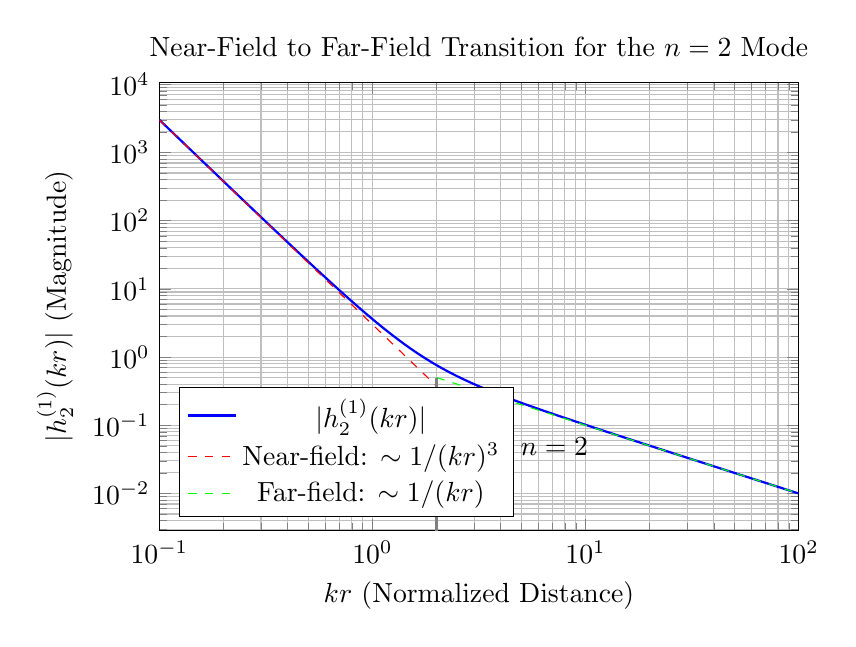
\begin{tikzpicture}
\begin{loglogaxis}[
    width=0.8\textwidth,
    height=0.6\textwidth,
    xlabel={$kr$ (Normalized Distance)},
    ylabel={$|h_2^{(1)}(kr)|$ (Magnitude)},
    title={Near-Field to Far-Field Transition for the $n=2$ Mode},
    grid=both,
    xmin=0.1, xmax=100,
    legend pos=south west,
]
% Data for |h_2(x)| = sqrt(( (x^2-3)/x^3*sin(x) - 3/x^2*cos(x) )^2 + ( -(x^2-3)/x^3*cos(x) - 3/x^2*sin(x) )^2)
% This simplifies to sqrt( (9+3*x^2+x^4)/x^6 )
\addplot[domain=0.1:100, samples=200, blue, thick] {sqrt((9+3*x^2+x^4)/x^6)};
\addlegendentry{$|h_2^{(1)}(kr)|$}

% Asymptotic Lines
\addplot[domain=0.1:2, samples=2, red, dashed] {3/x^3};
\addlegendentry{Near-field: $\sim 1/(kr)^3$}

\addplot[domain=2:100, samples=2, green, dashed] {1/x};
\addlegendentry{Far-field: $\sim 1/(kr)$}

% Transition Point
\draw[gray, thick] (axis cs:2,0.5) -- (axis cs:2, 0.001);
\node[anchor=west] at (axis cs:2.2, 0.05) {$kr \approx n = 2$};

\end{loglogaxis}
\end{tikzpicture}
\caption{Log-log plot of the magnitude of the $n=2$ spherical Hankel function. In the reactive near-field ($kr \ll 2$), the magnitude decays as $1/(kr)^3$. In the radiative far-field ($kr \gg 2$), it decays as $1/kr$. The transition occurs around $kr=n=2$.}
\end{figure}

\section{Maximum Gain and Supergain}

Harrington's theorem (1958) states that an antenna whose fields are composed of spherical modes up to degree $N$ has a maximum possible gain of:
\[
G_{\max}=N(N+2),\quad N\ge1.
\]
This implies that by exciting arbitrarily high modes ($N\to\infty$), one could achieve infinite gain. This is the principle of \textbf{supergain}. Substituting our relation $N \approx ka-\tfrac12$ from \eqref{eq:reactive_radius} connects the maximum gain to the electrical size of the reactive zone:
\[
G\approx\left(ka-\tfrac12\right)\left(ka+\tfrac32\right)
=(ka)^2+ka-\tfrac34.
\]
An antenna is considered superdirective if its gain $G$ exceeds the standard gain for its physical size $a_0$. This requires making the reactive radius $a$ much larger than the physical radius $a_0$, which leads to extreme stored energy and is very difficult in practice.

\section{Time-Domain Far Fields}

Introducing frequency dependence, the Rayleigh distance becomes $R_\omega=8\,a_\omega^2/\lambda$. By taking the Fourier transform of the frequency-domain far-field expression, we find the time-domain equivalent:
\[
E(r,\theta,\phi,t)\approx \frac{1}{r}\,F\left(\theta,\phi,t-\frac{r}{c}\right),
\quad \text{for } r\gtrsim \max_\omega R_\omega.
\]
For any real source, the signal is effectively bandlimited, meaning there is a maximum relevant frequency. This ensures that $\max_\omega R_\omega$ is finite. Therefore, the far-field pulses from all practical, finite-extent sources must eventually decay as $1/r$.

\section{Classical Photon Wavepackets}

While non-decaying pulses are impossible for finite-energy sources, the paper shows that quasi-localized wavepackets can exist for limited distances. A general wavepacket can be written as a superposition of plane waves:
\[
E(\vb r,t) = 2\Re\int \mathcal{E}(\vb k)e^{i(\vb k\cdot\vb r-\omega(\vb k)t)}\,d^3k, \quad \text{where }\omega(\vb k)=c|\vb k|
\]
If the spectrum $\mathcal{E}(\vb k)$ is concentrated around a central wavevector $\vb k_0=k_0\hat z$, we can approximate the integral to show that the wavepacket is a carrier wave modulated by a slow-varying envelope $g$:
\[
E(\vb r,t)\approx \Re\Bigl[g(\vb r-c\,t\hat z)\,e^{i(k_0z-\omega_0t)}\Bigr].
\]
The envelope $g$ travels at the speed of light $c$ without changing shape (in this approximation). By choosing a Gaussian spectrum, one can produce a Gaussian envelope confined to a volume of about one cubic wavelength. This is the paper's model for a ``classical photon.''

\section{Quantum-Classical Scattering Threshold}

This classical model can predict when quantum effects become important. We equate the energy density of a classical plane wave to the average energy density of a sea of photons:
\[
n_{\rm ph}\,\hbar\omega_0 = \frac12\epsilon_0E_0^2 = \frac{I_0}{c} \implies \text{mean spacing }d_{\rm ph}=n_{\rm ph}^{-1/3}.
\]
A classical field can be considered a smooth continuum when the constituent "photons" overlap. This requires their mean spacing to be smaller than their effective size, $\lambda_0$. Using the criterion $d_{\rm ph}\lesssim \lambda_0/4$:
\[
n_{\rm ph} \gtrsim \left(\frac{\lambda_0}{4}\right)^{-3} \implies \frac{\epsilon_0E_0^2}{2\hbar\omega_0} \gtrsim \frac{64}{\lambda_0^3}
\]
Rearranging this gives the final condition for the field to be treated classically:
\[
\frac{\epsilon_0E_0^2\lambda_0^3}{2} \gtrsim 64\hbar\omega_0
\]
This states that the classical energy within a cubic wavelength must be significantly larger than the energy of a single photon. This remarkable result, derived from a classical model, agrees with the rigorous condition from Quantum Electrodynamics (QED).

\subsection{Worked Example: Sunlight on Earth}
Is visible sunlight, which seems very bright, a classical field or a quantum stream of photons?
\begin{itemize}
    \item \textbf{Data:} The irradiance of sunlight is about $I_0 \approx 150 \text{ W/m}^2$ for a 100 nm bandwidth in the visible spectrum. We'll use green light with $\lambda_0 = 550 \text{ nm}$.
    \item \textbf{Photon Energy:} $E_{ph} = \hbar\omega_0 = hc/\lambda_0 \approx 3.6 \times 10^{-19} \text{ J}$.
    \item \textbf{Classical Energy Density:} $u_{EM} = I_0/c = 150 / (3 \times 10^8) = 5 \times 10^{-7} \text{ J/m}^3$.
    \item \textbf{Photon Number Density:} $n_{ph} = u_{EM} / E_{ph} \approx 1.4 \times 10^{12} \text{ photons/m}^3$.
    \item \textbf{Threshold Density:} For the field to be classical, we need $n_{ph} \gtrsim 64/\lambda_0^3$.
    \[ \frac{64}{\lambda_0^3} = \frac{64}{(550 \times 10^{-9})^3} \approx 3.8 \times 10^{20} \text{ photons/m}^3 \]
\end{itemize}
\textbf{Conclusion:} Since $1.4 \times 10^{12} \ll 3.8 \times 10^{20}$, the condition for classical behavior is strongly violated. Sunlight is a very dilute stream of photons. The detection of light by our eyes is fundamentally a quantum process, with individual photons triggering photoreceptor cells.

\appendix
\section{A Beginner's Guide to Compiling This Document}
\subsection{What is \LaTeX?}
\LaTeX\ is a document preparation system for high-quality typesetting. It is the standard for scientific and mathematical documents because of its superb control over formatting and equations.

\subsection{Required Software}
To compile this document, you need a TeX distribution. This is the backend engine that turns your `.tex` code into a PDF.
\begin{itemize}
    \item \textbf{Windows:} MiKTeX
    \item \textbf{macOS:} MacTeX
    \item \textbf{Linux:} TeX Live
\end{itemize}
You will also want a dedicated editor. Good options include TeXstudio, VS Code with the \texttt{LaTeX Workshop} extension, or online platforms like Overleaf (which require no installation).

\subsection{How to Compile}
\begin{enumerate}
    \item Save this code in a plain text file with a `.tex` extension (e.g., `yaghjian\_tutorial.tex`).
    \item Open a terminal or command prompt and navigate to the file's directory.
    \item Run the `pdflatex` command:
    \begin{verbatim}
    pdflatex yaghjian_tutorial.tex
    \end{verbatim}
    \item You may need to run the command two or three times. \LaTeX\ builds the document in passes: the first pass writes the content, the second pass generates the table of contents and cross-references, and a third pass ensures all references are correct.
\end{enumerate}


\end{document}